\chapter{Concatenação de subsequências}
\thispagestyle{empty}
O Problema da Mínima Latência (\textit{Minimum Latency Problem}, MLP) \referencia{} e o Problema de Roteamento de Veículos com Janelas de Tempo (\textit{Vehicle Routing Problem with Time Windows}, VRPTW) \referencia{} são exemplos problemas de otimização combinatória mais difíceis que o TSP. Parte dessas dificuldade reside em características especiais desses problemas, seja em termos de função objetivo ou de restrições. Tais diferenças tornam dificil avaliar o impacto de modificações na solução. No MLP, por exemplo, a aplicação de um movimento como o \textit{swap} pode alterar drasticamente o seu valor objetivo, que não pode mais ser calculado apenas somando e subtraindo custos de arestas, como no caso do TSP. No VRPTW, aplicar o mesmo movimento pode violar restrições do problema, exigindo uma avaliação prévia da sua viabilidade, que pode demandar muitas operações.

Reavaliar o custo de movimentos ou checar a viabilidade de novas soluções durante as buscas locais de forma ingênua pode comprometer e, por vezes, inviabilizar o método. Este capítulo aborda o método de concatenação de subsequências, que permite realizar essas avaliações de maneira eficiente para uma vasta classe de problemas. Para isso, a aplicação do método será apresentada para o MLP e o VRPTW, definidos nas seções seguintes. Ao fim do capítulo, espera-se que o leitor seja capaz de empregar as mesmas técnicas do capítulo anterior para esses problemas de forma eficiente.

\section{MLP}
Seja \(G = (V, E)\) um grafo em que cada aresta $\{\sigma_i, \sigma_j\} \in E$ está associada a um custo \(t_{{\sigma_i}{\sigma_j}}\). Suponha, ainda, que $|V| = n$ e que o \textit{tour} $s = (\sigma_1, \dots, \sigma_{n+1})$ é a sequência de vértices de um ciclo hamiltoniano em $G$, que começa e termina no nó $\sigma_1 = \sigma_{n+1}$. Considera-se $l(i) = \sum_{j=1}^{i-1} t_{{\sigma_j}{\sigma_{j+1}}}$ a ``latência'' $i$-ésimo nó da sequência $s$. Em outras palavras, se $t_{{\sigma_i}{\sigma_j}}$ é o tempo de viagem entre os nós $\sigma_i$ e $\sigma_j$, então $l(i)$ pode ser pensado como o tempo total de viagem do início do \textit{tour} $\sigma_1$ até o nó $\sigma_i$. Assim, se \(s = (1,3,6,2,4,7,5,1)\), por exemplo, então \[l(4) = t_{{1}{3}} + t_{{3}{6}} + t_{{6}{2}}\] é a latência do nó $\sigma_4 = 2$. O MLP visa encontrar um ciclo hamiltoniano $s$ em $G$ cuja latência total --- ou custo acumulado ---  \(f(s) = \sum_{i = 1}^{n+1} l(i) \) é mínima. 

Para compreender a motivação do problema, considere que um motorista deseja realizar uma sequência de entregas para $n$ clientes distintos. Para encontrar uma rota satisfatória em termos de tempo de viagem, o entregador poderia tratar o seu problema como um TSP, visando minimizar o custo total da própria viagem. Para satisfazer os clientes (i.e., realizar as entregas em um tempo razoável para todos eles), por outro lado, o entregador poderia tratar o problema como um MLP, tentando minimizar o tempo de entrega de cada um. Nesse caso, a latência $l(i)$ pode ser vista como o tempo necessário para realizar a entrega do $i$-ésimo cliente. Portanto, numa abordagem mais ``altruísta'', o MLP busca minimizar a soma de todos os tempos de entrega (latências). 

Por ter uma estrutura similar à do TSP, o problema pode ser abordado com o mesmo método baseado em busca local do capítulo anterior. Observe, porém, que a aplicação de qualquer um dos movimentos mostrados acarretaria drásticas mudanças no custo acumulado. Isso ocorre porque, diferente do caso do TSP, modificar um segmento no \textit{tour} implica em alterar a latência de todos os nós seguintes, que dependem diretamente da disposição dos nós anteriores. Dito isso, as próximas seções descrevem uma maneira de recalcular o custo acumulado em um número constante de operações.

%Considerando ainda o exemplo de sequência anterior, se uma nova solução \(\sigma' = (0,3,6,2,5,1,4,0)\) fosse obtida através da troca entre o quinto e sétimo nós, os valores de latência $l(5)$, $l(6)$, $l(7)$ e $l(8)$ seriam todos modificados. Consequentemente, a latência total \(f(\sigma')\) pode mudar drasticamente.

\subsection{Subsequências}
Seja \(s = (\sigma_1, \dots, \sigma_{n+1})\) uma solução viável para uma instância do MLP. Uma subsequência é uma sequência \(\sigma = (\sigma_i, \dots, \sigma_j)\), em que \(i, j \in \{1,\dots, n+1\}\). Além disso, considera-se $C(\sigma) = \sum_{k=i}^{j} l(\sigma_k)$ o custo acumulado da subsequência $\sigma$. Note que o número total de subsequências associadas a $s$, dentre as quais constam até mesmo sequências compostas por um único nó, é $(n+1)^2$.

\subsection{Concatenação de subsequências}
Sejam \(\sigma' = (\sigma'_1,\dots, \sigma'_a)\) e \(\sigma'' = (\sigma''_1, \dots, \sigma''_b)\) duas subsequências. A subsequência
\begin{align*}
    \sigma &= \sigma' \oplus \sigma'' \\
    &= (\sigma'_1,\dots,\sigma'_a,\sigma''_1,\dots,\sigma''_b)
\end{align*}
é resultado da concatenação de $\sigma'$ e $\sigma''$. A utilidade da concatenação de subsequências pode ser vista na Figura \ref{fig:quebraSubseq}, na qual o movimento \textit{swap} é aplicado entre os nós $\sigma_k$ e $\sigma_l$ de uma solução. A aplicação do movimento pode ser compreendida como a ``quebra'' da sequência da solução em um número fixo de subsequências --- 5 neste caso ---, que são então rearranjadas e concatenadas para formar uma nova solução. Todos os outros movimentos mostrados no capítulo anterior também podem ser vistos da mesma forma\footnote{Observe que as subsequências podem ter a sua ordem invertida. Isso ocore no caso do movimento \textit{2-opt}, que divide a solução em três subsequências, inverte uma delas, e as concatena novamente para formar uma nova solução.}. Em outras palavras, se uma maneira eficiente de calcular o custo acumulado de uma subsequência obtida após a concatenação de outras duas subsequências for conhecida, o impacto dos movimentos de várias estruturas de vizinhança herdadas do TSP também poderá ser facilmente avaliado, permitindo que sejam reutilizadas.

\begin{figure}
    \centering
   \scalebox{0.85}{
    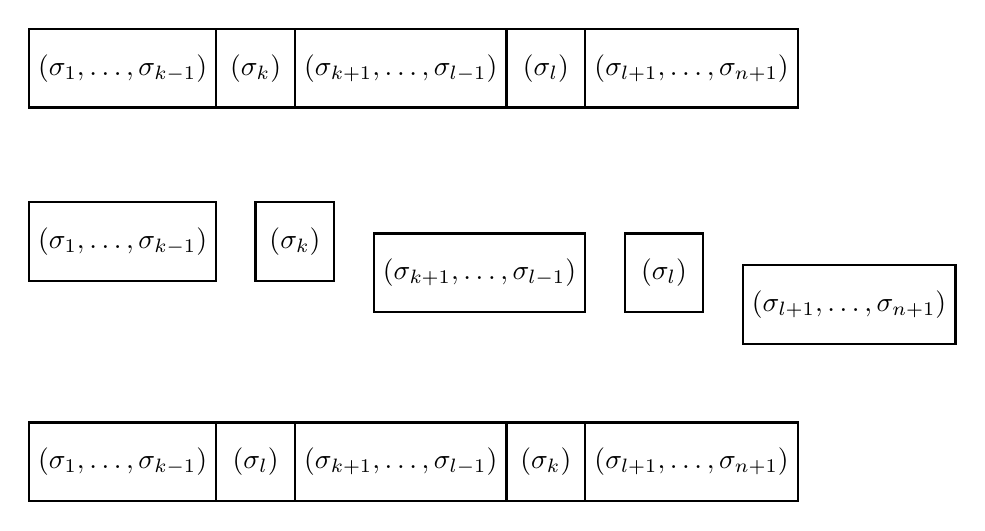
\begin{tikzpicture}
    % \node[rectangle, draw = black, minimum height = 1cm, outer sep = 0pt, minimum width = 1cm, thick] (1) at (-0.5,0.5) {$(\sigma_1, \dots, \sigma_{n+1})$};
    \node[rectangle, draw = black, minimum height = 1cm, outer sep = 0pt, minimum width = 1cm, thick] (a1) at (-0.5,0.5) {$(\sigma_1, \dots, \sigma_{k-1})$};
    \node[rectangle, draw = black, minimum height = 1cm, outer sep = 0pt, minimum width = 1cm, thick, anchor=west] (a2) at (a1.east) {$(\sigma_k)$};
    \node[rectangle, draw = black, minimum height = 1cm, outer sep = 0pt, minimum width = 1cm, thick, anchor=west] (a3) at (a2.east) {$(\sigma_{k+1}, \dots, \sigma_{l-1})$};
    \node[rectangle, draw = black, minimum height = 1cm, outer sep = 0pt, minimum width = 1cm, thick, anchor=west] (a4) at (a3.east) {$(\sigma_l)$};
    \node[rectangle, draw = black, minimum height = 1cm, outer sep = 0pt, minimum width = 1cm, thick, anchor=west] (a5) at (a4.east) {$(\sigma_{l+1}, \dots, \sigma_{n+1})$};
    
    \node[rectangle, draw = black, minimum height = 1cm, outer sep = 0pt, minimum width = 1cm, thick]              (b1) at ([yshift=-0.2cm]-0.5,-1.5) {$(\sigma_1, \dots, \sigma_{k-1})$};
    \node[rectangle, draw = black, minimum height = 1cm, outer sep = 0pt, minimum width = 1cm, thick, anchor=west] (b2) at ([xshift=0.5cm, yshift=0.2cm - 0.2cm] b1.east) {$(\sigma_k)$};
    \node[rectangle, draw = black, minimum height = 1cm, outer sep = 0pt, minimum width = 1cm, thick, anchor=west] (b3) at ([xshift=0.5cm, yshift=-0.2cm - 0.2cm] b2.east) {$(\sigma_{k+1}, \dots, \sigma_{l-1})$};
    \node[rectangle, draw = black, minimum height = 1cm, outer sep = 0pt, minimum width = 1cm, thick, anchor=west] (b4) at ([xshift=0.5cm, yshift=0.2cm - 0.2cm] b3.east) {$(\sigma_l)$};
    \node[rectangle, draw = black, minimum height = 1cm, outer sep = 0pt, minimum width = 1cm, thick, anchor=west] (b5) at ([xshift=0.5cm, yshift=-0.2cm - 0.2cm] b4.east) {$(\sigma_{l+1}, \dots, \sigma_{n+1})$};
    
    \node[rectangle, draw = black, minimum height = 1cm, outer sep = 0pt, minimum width = 1cm, thick]              (c1) at (-0.5,-4.5) {$(\sigma_1, \dots, \sigma_{k-1})$};
    \node[rectangle, draw = black, minimum height = 1cm, outer sep = 0pt, minimum width = 1cm, thick, anchor=west] (c2) at (c1.east) {$(\sigma_l)$};
    \node[rectangle, draw = black, minimum height = 1cm, outer sep = 0pt, minimum width = 1cm, thick, anchor=west] (c3) at (c2.east) {$(\sigma_{k+1}, \dots, \sigma_{l-1})$};
    \node[rectangle, draw = black, minimum height = 1cm, outer sep = 0pt, minimum width = 1cm, thick, anchor=west] (c4) at (c3.east) {$(\sigma_k)$};
    \node[rectangle, draw = black, minimum height = 1cm, outer sep = 0pt, minimum width = 1cm, thick, anchor=west] (c5) at (c4.east) {$(\sigma_{l+1}, \dots, \sigma_{n+1})$};
    \end{tikzpicture}
    }
    \caption{Quebra de uma solução em 5 subsequências e reconstrução durante o movimento \textit{swap}.}
    \label{fig:quebraSubseq}
\end{figure}


Para compreender como isso pode ser feito, observe a Figura \ref{fig:subseqConcat}, que ilustra a concatenação de duas subsequências $\sigma'$ e $\sigma''$ de tamanhos arbitrários $a\geq 1$ e $b\geq 1$, respectivamente. Na Figura \ref{fig:antesConcat}, as duas subsequências, bem como seus  custos acumulados $f(\sigma')$ e $f(\sigma'')$, escritos de forma explícita, são exibidos. Enquanto isso, o custo acumulado da subsequência $\sigma = \sigma' \oplus \sigma''$ é mostrado de forma similar na Figura \ref{fig:depoisConcat}. Note que tanto $f(\sigma')$ quanto $f(\sigma'')$ reaparecem no cálculo de $f(\sigma)$, sendo acompanhados pelo termo
\[ \Delta = t_{\sigma'_1 \sigma'_2} + \cdots + t_{\sigma'_{a-1} \sigma'_a} + t_{\sigma'_a \sigma''_1}, \]
que aparece $b$ vezes na soma. Isso significa que se $f(\sigma')$, $f(\sigma'')$ e $\Delta$ forem conhecidos previamente, pode-se calcular o custo acumulado da subsequência resultante da concatenação como
\[ f(\sigma) = f(\sigma') + b \Delta + f(\sigma''). \]

\begin{figure}[htpb!]
    \centering
    \begin{subfigure}{\textwidth}
\scalebox{0.75}{
    \begin{tikzpicture}[remember picture]
    \node[rectangle, draw = black, minimum height = 1cm, outer sep = 0pt, fill=blue!30, minimum width = 1cm, thick] (a1) at (-1.5,6) {$\sigma_1$};
    \node[rectangle, draw = black, minimum height = 1cm, outer sep = 0pt, fill=blue!30, minimum width = 1cm, thick, anchor=west] (a2) at (a1.east) {$\sigma_2$};
    \node[rectangle, draw = black, minimum height = 1cm, outer sep = 0pt, fill=blue!30, minimum width = 2cm, thick, anchor=west] (a3) at (a2.east) {$\cdots$};
    \node[rectangle, draw = black, minimum height = 1cm, outer sep = 0pt, fill=blue!30, minimum width = 1cm, thick, anchor=west] (a4) at (a3.east) {$\sigma_{a-1}$};
    \node[rectangle, draw = black, minimum height = 1cm, outer sep = 0pt, fill=blue!30, minimum width = 1cm, thick, anchor=west] (a5) at (a4.east) {$\sigma_a$};
    
    \node[rectangle, draw = black, minimum height = 1cm, outer sep = 0pt, fill=red!30, minimum width = 1cm, thick] (a6) at (6.5,5.5) {$\sigma_1$};
    \node[rectangle, draw = black, minimum height = 1cm, outer sep = 0pt, fill=red!30, minimum width = 1cm, thick, anchor=west] (a7) at (a6.east) {$\sigma_2$};
    \node[rectangle, draw = black, minimum height = 1cm, outer sep = 0pt, fill=red!30, minimum width = 1cm, thick, anchor=west] (a8) at (a7.east) {$\sigma_3$};
    \node[rectangle, draw = black, minimum height = 1cm, outer sep = 0pt, fill=red!30, minimum width = 2cm, thick, anchor=west] (a9) at (a8.east) {$\dots$};
    \node[rectangle, draw = black, minimum height = 1cm, outer sep = 0pt, fill=red!30, minimum width = 1cm, thick, anchor=west] (a10) at (a9.east) {$\sigma_{b-2}$};
    \node[rectangle, draw = black, minimum height = 1cm, outer sep = 0pt, fill=red!30, minimum width = 1cm, thick, anchor=west] (a11) at (a10.east) {$\sigma_{b-1}$};
    \node[rectangle, draw = black, minimum height = 1cm, outer sep = 0pt, fill=red!30, minimum width = 1cm, thick, anchor=west] (a12) at (a11.east) {$\sigma_b$};
    
    \draw[decorate,decoration={brace,amplitude=10pt, mirror}, ultra thick] ([yshift=-0.25cm, xshift=0.125cm] a1.south west) -- ([yshift=-0.25cm, xshift=-0.125cm] a5.south east) node[xshift=0, yshift=-0.75cm, midway]{\Large{$\sigma'$}};
    \draw[decorate,decoration={brace,amplitude=10pt, mirror}, ultra thick] ([yshift=-0.25cm, xshift=0.125cm] a6.south west) -- ([yshift=-0.25cm, xshift=-0.125cm] a12.south east) node[xshift=0, yshift=-0.75cm, midway]{\Large{$\sigma''$}};
    
    
    \node[rectangle, draw = black, draw opacity = 1, anchor=north west, fill=blue!30, above = of a3, rounded corners] (b1) {$\begin{aligned}
       &t_{\sigma'_1 \sigma'_2} + \\
       &\quad \vdots \\
        &+t_{\sigma'_1 \sigma'_2} + \cdots + t_{\sigma'_{a-1} \sigma'_{a}}\\
    \end{aligned}$};
    
    \node[rectangle, draw = black, draw opacity = 1, anchor=north west, fill=red!30, above = of a9, rounded corners] (b2) {$\begin{aligned}
       &t_{\sigma''_1 \sigma''_2} \\
        &+t_{\sigma''_1 \sigma''_2} + t_{\sigma''_{2} \sigma''_{3}} \\
       &\quad\quad \vdots \\
        &+t_{\sigma''_1 \sigma''_2} + t_{\sigma''_2 \sigma''_3} + \cdots + t_{\sigma''_{a-2} \sigma''_{a-1}}\\
        &+t_{\sigma''_1 \sigma''_2} + t_{\sigma''_2 \sigma''_3} + \cdots + t_{\sigma'_{a-2} \sigma'_{a-1}} + t_{\sigma'_{a-1} \sigma'_{a}}\\
    \end{aligned}$};
    
    \draw[decorate,decoration={brace,amplitude=5pt,mirror}, ultra thick] ([xshift=-0.125cm] b1.north west) -- ([xshift=-0.125cm] b1.south west) node[xshift=-1cm, midway]{{$f(\sigma')$}};
    \draw[decorate,decoration={brace,amplitude=5pt,mirror}, ultra thick] ([xshift=-0.125cm] b2.north west) -- ([xshift=-0.125cm] b2.south west) node[xshift=-1cm, midway]{{$f(\sigma'')$}};
    
    
    
    \end{tikzpicture}
    }
    \caption{Antes da concatenação.}
    \label{fig:antesConcat}
    \end{subfigure}
    \begin{subfigure}{\textwidth}
\scalebox{0.75}{
    \begin{tikzpicture}[remember picture]
    \node[rectangle, draw = black, minimum height = 1cm, outer sep = 0pt, fill=blue!30, minimum width = 1cm, thick] (1) at (-0.5,0.5) {$\sigma'_1$};
    \node[rectangle, draw = black, minimum height = 1cm, outer sep = 0pt, fill=blue!30, minimum width = 1cm, thick, anchor=west] (2) at (1.east) {$\sigma'_2$};
    \node[rectangle, draw = black, minimum height = 1cm, outer sep = 0pt, fill=blue!30, minimum width = 2cm, thick, anchor=west] (3) at (2.east) {$\cdots$};
    \node[rectangle, draw = black, minimum height = 1cm, outer sep = 0pt, fill=blue!30, minimum width = 1cm, thick, anchor=west] (4) at (3.east) {$\sigma'_{a-1}$};
    \node[rectangle, draw = black, minimum height = 1cm, outer sep = 0pt, fill=blue!30, minimum width = 1cm, thick, anchor=west] (5) at (4.east) {$\sigma'_a$};
    
    \node[rectangle, draw = black, minimum height = 1cm, outer sep = 0pt, fill=red!30, minimum width = 1cm, thick, anchor=west] (6) at (5.east) {$\sigma''_1$};
    \node[rectangle, draw = black, minimum height = 1cm, outer sep = 0pt, fill=red!30, minimum width = 1cm, thick, anchor=west] (7) at (6.east) {$\sigma''_2$};
    \node[rectangle, draw = black, minimum height = 1cm, outer sep = 0pt, fill=red!30, minimum width = 1cm, thick, anchor=west] (8) at (7.east) {$\sigma''_3$};
    \node[rectangle, draw = black, minimum height = 1cm, outer sep = 0pt, fill=red!30, minimum width = 2cm, thick, anchor=west] (9) at (8.east) {$\dots$};
    \node[rectangle, draw = black, minimum height = 1cm, outer sep = 0pt, fill=red!30, minimum width = 1cm, thick, anchor=west] (10) at (9.east) {$\sigma''_{b-2}$};
    \node[rectangle, draw = black, minimum height = 1cm, outer sep = 0pt, fill=red!30, minimum width = 1cm, thick, anchor=west] (11) at (10.east) {$\sigma''_{b-1}$};
    \node[rectangle, draw = black, minimum height = 1cm, outer sep = 0pt, fill=red!30, minimum width = 1cm, thick, anchor=west] (12) at (11.east) {$\sigma''_b$};
    
    \draw[decorate,decoration={brace,amplitude=10pt}, ultra thick] ([yshift=0.25cm, xshift=0.125cm] 1.north west) -- ([yshift=0.25cm, xshift=-0.125cm] 12.north east) node[xshift=0, yshift=1cm, midway]{\large{$\sigma = \sigma' \oplus \sigma''$}};
    
     \draw[dashed, fill = blue!30, rounded corners, fill opacity = 0.25, draw opacity = 1] ([yshift=10pt,xshift=-4pt] pic cs:a) rectangle ([xshift=2pt, yshift=-6pt]pic cs:b);
     \draw[fill=gray!20, rounded corners, fill opacity = 0.25] ([yshift=10pt,xshift=-2pt] pic cs:c) rectangle ([xshift=2pt, yshift=-6pt]pic cs:d);
     \draw[dashed, fill = red!30, rounded corners, fill opacity = 0.25, draw opacity = 1] ([yshift=10pt,xshift=-2pt] pic cs:e) rectangle ([xshift=2pt, yshift=-6pt]pic cs:f);
    
    \draw[decorate,decoration={brace,amplitude=5pt, mirror}, ultra thick] ([xshift=-0.25cm, yshift=0cm] pic cs:c) -- ([xshift=-0.25cm, yshift=-0cm] pic cs:i) node[xshift=-0.6cm, midway]{\large{$b\Delta$}};
    \draw[decorate,decoration={brace,amplitude=17pt, mirror}, ultra thick] ([xshift=-1cm, yshift=0.5cm] pic cs:a) -- ([xshift=-1cm, yshift=-0.25cm] pic cs:i) node[xshift=-1.5cm, midway]{\large{$f(\sigma)$}};
    
    \node[rectangle, below = 0.25cm of 12.east, outer sep = 0pt] (14) at (6,-1) {$\begin{aligned}
       & \tikzmark{a} t_{\sigma'_1 \sigma'_2} \\
       &\quad \vdots \\
        &\tikzmark{g} +t_{\sigma'_1 \sigma'_2} + \cdots + t_{\sigma'_{a-1} \sigma'_{a}} \tikzmark{b} \\
        &\tikzmark{c} + t_{\sigma'_1 \sigma'_2} +  \cdots + t_{\sigma'_{a-1} \sigma'_a} + t_{\sigma'_{a} \sigma''_1} \\
        &+ t_{\sigma'_1 \sigma'_2} +  \cdots + t_{\sigma'_{a-1} \sigma'_a} + t_{\sigma'_{a} \sigma''_1}  +   \tikzmark{e}  t_{\sigma''_1 \sigma''_2} \\
        &+t_{\sigma'_1 \sigma'_2} + \cdots + t_{\sigma'_{a-1} \sigma'_a} + t_{\sigma'_{a} \sigma''_1}  +  t_{\sigma''_1 \sigma''_2} + t_{\sigma''_{2} \sigma''_{3}} \\
        &\quad\vdots \\
        &+t_{\sigma'_1 \sigma'_2} + \cdots + t_{\sigma'_{a-1} \sigma'_a} + t_{\sigma'_{a} \sigma''_1}  +  t_{\sigma''_1 \sigma''_2} + t_{\sigma''_2 \sigma''_3} + \cdots + t_{\sigma''_{b-2} \sigma''_{b-1}} \\
        &\tikzmark{i} + t_{\sigma'_1 \sigma'_2} + \cdots + t_{\sigma'_{a-1} \sigma'_a} + t_{\sigma'_{a} \sigma''_1} \tikzmark{d}   +  \tikzmark{h} t_{\sigma''_1 \sigma''_2} + t_{\sigma''_2 \sigma''_3} + \cdots + t_{\sigma'_{b-2} \sigma'_{b-1}} + t_{\sigma'_{b-1} \sigma'_{b}} \tikzmark{f} \\
    \end{aligned}$};
    
    %\draw[decorate,decoration={brace,amplitude=10pt, mirror}, ultra thick] ([yshift=-0.25cm, xshift=0.125cm] a1.south west) -- ([yshift=-0.25cm, xshift=-0.125cm] a5.south east) node[xshift=0, yshift=-0.75cm, midway]{\large{$\sigma'$}};
    %\draw[decorate,decoration={brace,amplitude=10pt, mirror}, ultra thick] ([yshift=-0.25cm, xshift=0.125cm] a6.south west) -- ([yshift=-0.25cm, xshift=-0.125cm] a12.south east) node[xshift=0, yshift=-0.75cm, midway]{\large{$\sigma''$}};
    %
    \end{tikzpicture}
    }
    \caption{Após a concatenação.}
    \label{fig:depoisConcat}
    \end{subfigure}
    \caption{Concatenação de duas subsequências $\sigma'$ e $\sigma''$.}
    \label{fig:subseqConcat}
\end{figure}



\subsection{Estruturas auxiliares}

Sejam $s = (\sigma_1, \dots, \sigma_{n+1})$ uma solução viável qualquer para uma instância do MLP, e $\sigma$ uma subsequência de $s$. Além de seu custo acumulado $C(\sigma)$, a subsequência $\sigma$ também é caracterizada pelos valores auxiliares $W(\sigma)$ (custo de atraso) e $T(\sigma)$ (duração). Caso $\sigma$ seja uma subsequência composta por um único nó, 
\begin{align}
    &T(\sigma) = 0, \label{duracaoEqSimples} \\
    &C(\sigma) = 0, \label{custoAcumuladoEqSimples} \\
    &W(\sigma) = \begin{cases} 0 \text{ se } \sigma = (\sigma_1), \\ 1 \text{ caso contrário.} \end{cases} \label{custoDeAtrasoEqSimples}
\end{align}
Se, por outro lado, $\sigma$ for resultado da concatenação de outras duas subsequências $\sigma'$ e $\sigma''$, então 
\begin{align}
    &T(\sigma' \oplus \sigma'') = T(\sigma') + t_{{\sigma'_a}{\sigma''_1}} +  T(\sigma''),  \label{duracaoEq} \\
    &C(\sigma' \oplus \sigma'') = C(\sigma') + W(\sigma'')\left( T(\sigma') + t_{{\sigma'_a}{\sigma''_1}} \right) +  C(\sigma''), \label{custoAcumuladoEq}\\
    &W(\sigma' \oplus \sigma'') = W(\sigma') + W(\sigma'') \label{custoDeAtrasoEq}.
\end{align}

Conforme explicado na seção anterior, a equação \eqref{custoAcumuladoEq} descreve o cálculo do custo acumulado da subsequência resultante a partir dos custos das duas subsequências envolvidas na operação de concatenação. Dessa forma, se $T(\sigma)$, $C(\sigma)$ e $W(\sigma)$ forem conhecidos previamente para todas as subsequências $\sigma$ possíveis de uma solução $s$, qualquer outra solução vizinha $s'$ obtida aplicando-se um dos movimentos do capítulo anterior pode ter seu custo facilmente avaliado através de algumas operações de soma. 

\subsubsection{Representação das estruturas auxiliares}

O trecho de código a seguir mostra como as informações relevantes de uma subsequência podem ser armazenados. Além dos valores já mostrados, o primeiro e último nós (\texttt{first} e \texttt{last}, respectivamente) de cada subsequência também devem ser armazenados para que se possa aplicar as equações \eqref{duracaoEq} e \eqref{custoAcumuladoEq}. A partir de duas subsequências \texttt{sigma\_1} e \texttt{sigma\_2}, a função \texttt{Concatenate()} aplica as equações \eqref{duracaoEq}--\eqref{custoDeAtrasoEq} e retorna a subsequência resultante \texttt{sigma}.

\begin{lstlisting}[style=cplusplusListStyle]
struct Subsequence
{
    double T, C;
    int W;
    int first, last; // primeiro e ultimo nos da subsequencia
    inline static Subsequence Concatenate(Subsequence &sigma_1, Subsequence &sigma_2)
    {
        Subsequence sigma;
        double temp = t[sigma_1.last][sigma_2.first];
        sigma.W = sigma_1.W + sigma_2.W;
        sigma.T = sigma_1.T + temp + sigma_2.T;
        sigma.C = sigma_1.C + sigma_2.W * (sigma_1.T + temp) + sigma_2.C;
        sigma.first = sigma_1.first;
        sigma.last = sigma_2.last;
        
        return sigma;
    }
};
\end{lstlisting}

\subsubsection{Inicialização das estruturas auxiliares}

O trecho de código a seguir mostra como os valores de todas as subsequências de uma solução podem ser inicializados. Os valores auxiliares de cada subsequência de uma solução são armazenados em \texttt{subseq\_matrix}. O elemento \texttt{subseq\_matrix[i][j]} armazena as informações da subsequência que começa no $i$-ésimo nó e termina no $j$-ésimo nó de \texttt{s}. No código, primeiramente, aplica-se as equações \eqref{duracaoEqSimples}--\eqref{custoDeAtrasoEqSimples} para que as subsequências formadas por apenas um nó sejam obtidas. Em seguida, as outras subsequências são obtidas por meio de operações de concatenação.

\begin{lstlisting}[style=cplusplusListStyle]
// n: numero de nos da instancia
// s: solucao corrente
// subseq_matrix = vector<vector<Subsequence>>(n, vector<Subsequence>(n));

void UpdateAllSubseq(Solution *s, vector<vector<Subsequence>> &subseq_matrix)
{
    int n = s->sequence.size();

    // subsequencias de um unico no
    for (int i = 0; i < n; i++)
    {
        int v = s->sequence[i];
        subseq_matrix[i][i].W = (i > 0);
        subseq_matrix[i][i].C = 0;
        subseq_matrix[i][i].T = 0;
        subseq_matrix[i][i].first = s->sequence[i];
        subseq_matrix[i][i].last = s->sequence[i];
    }
    
    for (int i = 0; i < n; i++)
        for (int j = i + 1; j < n; j++)
            subseq_matrix[i][j] = Subsequence::Concatenate(subseq_matrix[i][j-1], subseq_matrix[j][j]);
            
    // subsequencias invertidas
    // (necessarias para o 2-opt)
    for (int i = n - 1; i >= 0; i--)
        for (int j = i - 1; j >= 0; j--)
            subseq_matrix[i][j] = Subsequence::Concatenate(subseq_matrix[i][j+1], subseq_matrix[j][j]);
}
\end{lstlisting}

Após construir a matriz de subsequências a partir de uma solução inicial obtida através de um procedimento construtivo, pode-se, enfim, calcular o impacto de movimentos de maneira eficiente. Isso pode ser visto no trecho de código a seguir, no qual o custo de uma solução obtida após a aplicação do movimento \textit{2-opt} foi obtido utilizando-se duas operações de concatenação. O valor \texttt{sigma\_2.C} equivale ao custo acumulado da nova solução, que pode então ser comparado ao custo da solução anterior.

\begin{lstlisting}[style=cplusplusListStyle]
Solution *s = Construction(); 
subseq_matrix = vector<vector<Subsequence>>(n, vector<Subsequence>(n));
UpdateAllSubseq(s, subseq_matrix);
// movimento 2-opt remove as arestas {i-1, i} e {j, j+1}, 
// dividindo a solucao em tres subsequencias.
// no 2-opt a subsequencia que comeca em i e termina em j e invertida
// por isso, ela foi acessada por meio de subseq_matrix[j][i], e nao subseq_matrix[i][j]
Subsequence sigma_1 = Subsequence::Concatenate(subseq_matrix[0][i-1], subseq_matrix[j][i]);
Subsequence sigma_2 = Subsequence::Concatenate(sigma_1, subseq_matrix[j+1][n]);
if (sigma_2.C < s->cost)
{
    ApplyTwoOpt(s, i, j);
    // A solucao foi modificada,
    // logo, as subsequencias devem ser recalculadas
    UpdateAllSubseq(s, subseq_matrix);
}
\end{lstlisting}

\subsection{Atualização de subsequências}
Sempre que uma nova solução é criada, a matriz de subsequências deve ser computada a partir do zero, exigindo $(n+1)^2 - n - 1$ operações de concatenação. Quando uma solução é modificada por um movimento, no entanto, algumas subsequências permanecem inalteradas. Isso pode ser visto mais facilmente na Figura \ref{fig:atualizaSubseqMatrix}, que mostra a matriz de subsequências de uma solução $s = (\sigma_1, \dots, \sigma_{15})$ alterada por um movimento qualquer entre os nós $\sigma_9$ e $\sigma_{11}$. A região cinza na figura representa os elementos na matriz que precisam ser atualizados. Os elementos restantes, por sua vez, não precisam ser atualizados, já que as subsequências associadas não foram alteradas.

\begin{figure}
    \centering
   \scalebox{0.8}{
    \begin{tikzpicture}
    \foreach \i in {1,...,15}
    \foreach \j in {1,...,15}
    {
        \ifthenelse{\(\i < 9 \AND \j < 9\)  \OR \(\i > 11 \AND \j > 11\)}
        {
        \node[outer sep = 0, minimum width = 0.5cm, minimum height = 0.5cm, rectangle, draw = black, fill = white] (\i-\j) at (0.5*\j,-0.5*\i) {};
        }
        {
        \node[outer sep = 0, minimum width = 0.5cm, minimum height = 0.5cm, rectangle, draw = black, fill = gray!50] (\i-\j) at (0.5*\j,-0.5*\i) {};
        }
        %\ifthenelse{\i = \j}
        %{
        %\node[outer sep = 0, minimum width = 0.5cm, minimum height = 0.5cm, rectangle, draw = black, fill = gray!85] (\i-\j) at (0.5*\j,-0.5*\i) {};
        %} {}
    }
    
    \node[outer sep = 0, minimum width = 0.5cm, minimum height = 0.5cm, rectangle, draw = black, fill = white, ultra thick] at (0.5*6,-0.5*3) {};
    \node[outer sep = 0, minimum width = 0.5cm, minimum height = 0.5cm, rectangle, draw = black, fill = gray!50, ultra thick] at (0.5*5,-0.5*10) {};
    
    \node[rectangle, anchor=center, rectangle, draw = black] at (3.75,-8.5) {$s = (\sigma_1, \dots, \sigma_{15})$};
    \node[rectangle, anchor=center, align=center, rectangle, draw = black] (subseq1) at (-2.5, -3.5) {{\small\texttt{subseq\_matrix[10][5]}} \\ $(\sigma_{10}, \dots, \sigma_{5})$};
    \node[rectangle, anchor=center, align=center, rectangle, draw = black] (subseq2) at (3, 1) {{\small\texttt{subseq\_matrix[3][6]}} \\ $(\sigma_{3}, \dots, \sigma_{6})$};
    
    
    \draw[decorate,decoration={brace,amplitude=10pt}, ultra thick] (8.25, -0.5) -- (8.25, -7.5) node[xshift=2cm, midway]{{\small \texttt{subseq\_matrix}}};
    
    %\draw[-{Triangle}, rounded corners, line width = 0.05cm] (10-5.west) -| (subseq1.south);
    %\draw[-{Triangle}, rounded corners, line width = 0.05cm] (3-6.north) -- +(0,1) -| (subseq2.south);
    \draw[-, ultra thick, rounded corners] (10-5.west) -| (subseq1.south);
    \draw[-, ultra thick, rounded corners] (3-6.north) -- +(0,1) -| (subseq2.south);
    \end{tikzpicture}
    }
    \caption{Matriz de subsequências de uma solução.}
    \label{fig:atualizaSubseqMatrix}
\end{figure}

No geral, é sempre possível pensar em maneiras diferentes de atualizar a matriz de subsequências levando-se em conta as particularidades de cada movimento. Porém, isso exigiria a implementação de uma função de atualização de subsequências para cada movimento. Felizmente, a ideia mostrada na Figura \ref{fig:atualizaSubseqMatrix} é aplicável a qualquer movimento, apresentando um bom equilíbrio entre facilidade de implementação e impacto no tempo de execução do algoritmo.

\subsection{Aplicando o ILS ao MLP}
Uma algoritmo simples para resolver o MLP é descrito em \cite{SILVA2012513}. Para resolver o problema, os autores utilizaram a meta-heurística ILS. Com exceção do procedimento construtivo, mostrado no Algoritmo \ref{alg:mlpConstruction}, todos os procedimentos, incluindo perturbação, busca local e estruturas de vizinhança, foram implementados exatamente como descrito no capítulo anterior. Para fazer as buscas locais de maneira eficiente, as estruturas auxiliares descritas nas seções anteriores foram utilizadas. O algoritmo é um dos métodos heurísticos mais efetivos para resolver o MLP. Como exercício, o leitor é encorajado a replicá-lo. Para isso, convém utilizar como base o código desenvolvido no capítulo anterior, adicionando a estrutura \texttt{Subsequence} e a matriz de subsequências. Os resultados podem então ser comparados com os do artigo citado\footnote{Os autores do artigo utilizaram um subconjunto de instâncias do TSP. Portanto, o mesmo leitor leitor de instâncias pode ser usado.}.

\begin{algorithm}[!ht]
    \DontPrintSemicolon
    %\KwIn{Sequência $s$ e número de vértices $n$}
    %\KwOut{Sentence instances with cost-vectors for training $S_{i,c_i}$}
    % \tcp{Exemplo: s = \{1,5,4,3,6,2,1\}, n = 6}
    % \tcp{\(s_1\) = 1, \(s_2\) = 5, \(s_3\) = 4, ...}
    \SetKwBlock{Begin}{função}{end função}
   \caption{Construction} \label{alg:mlpConstruction}
   Procedure Construction($\alpha$)\\
    $s \gets \{1\}$\; \label{SI:solucao}
    Initialize Candidate List $CL$\; \label{SI:lista}
    $CL \leftarrow CL - \{1\}$\; \label{SI:listasemdeposito}
    $r \leftarrow 1$\;
    \While{$CL \neq \emptyset$}{ \label{SI:inicio}
     Sort $CL$ in ascending order according to their distance with respect to $r$\; \label{SI:ordena}
     $RCL \gets $ $\alpha \%$ best candidates of $CL$\; \label{SI:iniciaLRC}
     Choose $c \in RCL$ at random\; \label{SI:seleciona}
     $s \gets s \cup \{c\}$\; \label{SI:salva}
     $r \leftarrow c$\;
     $CL \leftarrow CL - \{r\}$\;
    } \label{SI:fim}
    \Return{$s$\;}
   end Construction
\end{algorithm}

A Tabela \ref{tab:mlpResults} contém os valores médios de custo acumulado e tempo (em segundos) de resolução das instâncias após 10 execuções do algoritmo em um Intel{\textregistered} Core{\texttrademark} i7 $2.93$ GHz. Durante os experimentos, os autores utilizaram os parâmetros $I_{Max} = 10$, $I_{ILS} = \min\{100,n\}$ e $R = \{0.00, 0.01, 0.02,\dots,0.25\}$.
 \begin{table}[!ht]
 \centering
 \caption{Resultados do método de \cite{SILVA2012513}.}
 \footnotesize
 \begin{tabular}{ccc}
 \toprule
\multirow{2.5}{*}{\textbf{Instância}} & \multicolumn{2}{c}{\textbf{Resultados}} \\
\cmidrule{2-3} & \textbf{Tempo} & \textbf{Custo} \\
\midrule
  \texttt{dantzig42}   & 0.16 & 12528.00 \\ 
  \texttt{swiss42}   & 0.16 & 22327.00 \\ 
  \texttt{att48}   & 0.32 & 209320.00 \\ 
  \texttt{gr48}   & 0.33 & 102378.00 \\ 
  \texttt{hk48}   & 0.30 & 247926.00 \\ 
  \texttt{eil51}   & 0.49 & 10178.00 \\ 
  \texttt{berlin52}   & 0.46 & 143721.00 \\ 
  \texttt{brazil58}   & 0.78 & 512361.00 \\ 
  \texttt{st70}   & 1.65 & 20557.00 \\ 
  \texttt{eil76}   & 2.64 & 17976.00 \\ 
  \texttt{pr76}   & 2.31 & 3455242.00 \\ 
  \texttt{pr76r}   & 2.41 & 345427.00 \\ 
  \texttt{gr96}   & 6.19 & 2097170.00 \\ 
  \texttt{rat99}   & 11.27 & {57986.00} \\ 
  \texttt{kroA100}   & 8.59 & 983128.00 \\ 
  \texttt{kroB100}   & 9.21 & 986008.00 \\ 
  \texttt{kroC100}   & 8.17 & 961324.00 \\ 
  \texttt{kroD100}   & 8.46 & 976965.00 \\ 
  \texttt{kroE100}   & 8.31 & 971266.00 \\ 
  \texttt{rd100}   & 8.52 & 340047.00 \\ 
  \texttt{eil101}   & 12.76 & {27513.00} \\ 
  \texttt{lin105}   & 8.42 & 603910.00 \\ 
  \texttt{pr107}   & 10.89 & 2026626.00 \\ 
\bottomrule
 \end{tabular}
 \label{tab:mlpResults}
 \end{table}
 
 
 

\section{VRPTW}
Seja $G = (V,A)$ um grafo direcionado em que $V$ e $A$ são os conjuntos de vértices e arcos, respectivamente. Tem-se que $V = V' \cup \{0\}$, onde o subconjunto $V' = \{1, \dots, n\}$ representa os clientes e o vértice $0$ é o depósito, e $A = \{ (i,j) \mid i \neq j \}$. O custo de viajar por um arco $(i,j)\in A$ é $c_{ij}$, e a matriz de custos satisfaz a desigualdade triangular. Cada vértice $i \in V$ possui um tempo de serviço $s_i$, uma janela de tempo $[w_i^a, w_i^b]$ e uma demanda $d_i$, sendo $d_0 = 0$. Há também um tempo de viagem $t_{ij}$ associado a cada arco $(i,j) \in A$. Dada uma frota homogênea e ilimitada de veículos de capacidade $C$, o problema consiste em determinar um conjunto de rotas de custo mínimo de modo que: (\textit{i}) cada rota deve começar no depósito, visitar um subconjunto dos clientes, e terminar no depósito; (\textit{ii}) a capacidade do veículo não pode ser excedida; (\textit{iii}) as janelas de tempo não devem ser violadas; (\textit{iv}) todo cliente deve ser visitado exatamente uma vez, tendo sua demanda suprida.

\subsection{Estruturas auxiliares}
